\subsection[STL]{The STL}

\begin{frame}[fragile]
  \frametitlecpp[98]{The Standard Template Library}
  \begin{block}{What it is}
    \begin{itemize}
    \item A library of standard templates
    \item Everything you need, or ever dreamed of
      \begin{itemize}
      \item strings, containers, iterators
      \item algorithms, functions, sorters
      \item functors, allocators
      \item ...
      \end{itemize}
    \item Portable
    \item Reusable
    \item Efficient
    \end{itemize}
  \end{block}
  \pause
  \begin{alertblock}{Just use it}
    and adapt it to your needs, thanks to templates
  \end{alertblock}
\end{frame}

\begin{frame}[fragile,label=STLcode]
  \frametitlecpp[14]{STL in practice}
  \begin{cppcode*}{}
    #include <vector>
    #include <algorithm>

    std::vector<int> vi{5, 3, 4}; // initializer list
    std::vector<int> vr(3); // constructor taking int

    std::transform(vi.begin(), vi.end(),      // range1
                   vi.begin(),          // start range2
                   vr.begin(),          // start result
                   std::multiplies{}); // function

    for(auto n : vr) {
      std::cout << n << ' ';
    }
  \end{cppcode*}
\end{frame}

\begin{frame}[fragile]
  \frametitlecpp[98]{STL's concepts}
  \begin{block}{containers}
    \begin{itemize}
    \item a structure containing data
    \item with a given way of handling it
    \item irrespective of
      \begin{itemize}
      \item the data itself (templated)
      \item the memory allocation of the structure (templated)
      \item the algorithms that may use the structure
      \end{itemize}
    \item examples
      \begin{itemize}
      \item string
      \item tuple, list, forward\_list (\cpp11), vector, deque, array (\cpp11)
      \item map, set, multimap, multiset
      \item unordered\_map (\cpp11), unordered\_set (\cpp11)
      \item stack, queue, priority\_queue
      \end{itemize}
    \end{itemize}
  \end{block}
\end{frame}

\begin{frame}[fragile]
  \frametitlecpp[98]{STL's concepts}
  \begin{block}{iterators}
    \begin{itemize}
    \item generalization of pointers
    \item allow iteration over some data
    \item irrespective of
      \begin{itemize}
      \item the container used (templated)
      \item the data itself (container is templated)
      \item the consumer of the data (templated algorithm)
      \end{itemize}
    \item examples
      \begin{itemize}
      \item iterator
      \item reverse\_iterator
      \item const\_iterator
      \end{itemize}
    \end{itemize}
  \end{block}
\end{frame}

\begin{frame}[fragile]
  \frametitlecpp[98]{STL's concepts}
  \begin{block}{algorithms}
    \begin{itemize}
    \item implementation of an algorithm working on data
    \item with a well defined behavior (defined complexity)
    \item irrespective of
      \begin{itemize}
      \item the data handled
      \item the container where the data live
      \item the iterator used to go through data (almost)
      \end{itemize}
    \item examples
      \begin{itemize}
      \item for\_each, find, find\_if, count, count\_if, search
      \item copy, swap, transform, replace, fill, generate
      \item remove, remove\_if
      \item unique, reverse, rotate, shuffle, partition
      \item sort, partial\_sort, merge, make\_heap, min, max
      \item lexicographical\_compare, iota, reduce, partial\_sum
      \end{itemize}
    \end{itemize}
  \end{block}
\end{frame}

\begin{frame}[fragile]
  \frametitlecpp[98]{STL's concepts}
  \begin{block}{functors / function objects}
    \begin{itemize}
      \item generic utility functions
      \item as structs with \mintinline{cpp}{operator()}
      \item mostly useful to be passed to STL algorithms
    \item implemented independently of
      \begin{itemize}
      \item the data handled (templated)
      \item the context (algorithm) calling it
      \end{itemize}
    \item examples
      \begin{itemize}
      \item plus, minus, multiplies, divides, modulus, negate
      \item equal\_to, less, greater, less\_equal, ...
      \item logical\_and, logical\_or, logical\_not
      \item bit\_and, bit\_or, bit\_xor, bit\_not
      \item identity, not\_fn
      \item bind, bind\_front
      \end{itemize}
    \end{itemize}
  \end{block}
\end{frame}

\againframe{STLcode}

\begin{frame}[fragile]
  \frametitlecpp[98]{STL in practice using \cpp98}
  \begin{cppcode*}{}
    #include <vector>
    #include <algorithm>

    std::vector<int> vi, vr(3);
    vi.push_back(5); vi.push_back(3); vi.push_back(4);

    std::transform(vi.begin(), vi.end(),      // range1
                   vi.begin(),          // start range2
                   vr.begin(),          // start result
                   std::multiplies<int>()); // function

    for(std::vector<int>::iterator it = vr.begin();
        it != vr.end();
        it++) {
      std::cout << *it << ' ';
    };
  \end{cppcode*}
\end{frame}

\begin{frame}[fragile]
  \frametitlecpp[98]{STL and functors}
  \begin{cppcode}
    // Finds the first element in a list between 1 and 10.
    list<int> l;
    ...
    list<int>::iterator it =
      find_if(l.begin(), l.end(),
              compose2(logical_and<bool>(),
                       bind2nd(greater_equal<int>(), 1),
                       bind2nd(less_equal<int>(), 10)));

    // Computes sin(x)/(x + DBL_MIN) for elements of a range.
    transform(first, last, first,
              compose2(divides<double>(), // non-standard
                       ptr_fun(sin),
                       bind2nd(plus<double>(), DBL_MIN)));
  \end{cppcode}
  \begin{alertblock}{Deprecation warning}
  	Binders and function adaptors were removed in \cpp17 or \cpp20
  \end{alertblock}
\end{frame}

\begin{frame}[fragile]
  \frametitlecpp[14]{STL and lambdas}
  \begin{cppcode}
    // Finds the first element in a list between 1 and 10.
    list<int> l;
    ...
    const auto it =
      find_if(l.begin(), l.end(),
        [](int i) { return i >= 1 && i <= 10; });

    // Computes sin(x)/(x + DBL_MIN) for elements of a range.
    transform(first, last, first,
      [](auto x) { return sin(x)/(x + DBL_MIN); });
  \end{cppcode}
\end{frame}

\begin{frame}[fragile]
  \frametitlecpp[98]{Welcome to lego programming !}
  \begin{block}{}
    \pgfdeclareimage[height=0.5cm]{AtlasLego}{morelanguage/AtlasLego.jpg}
    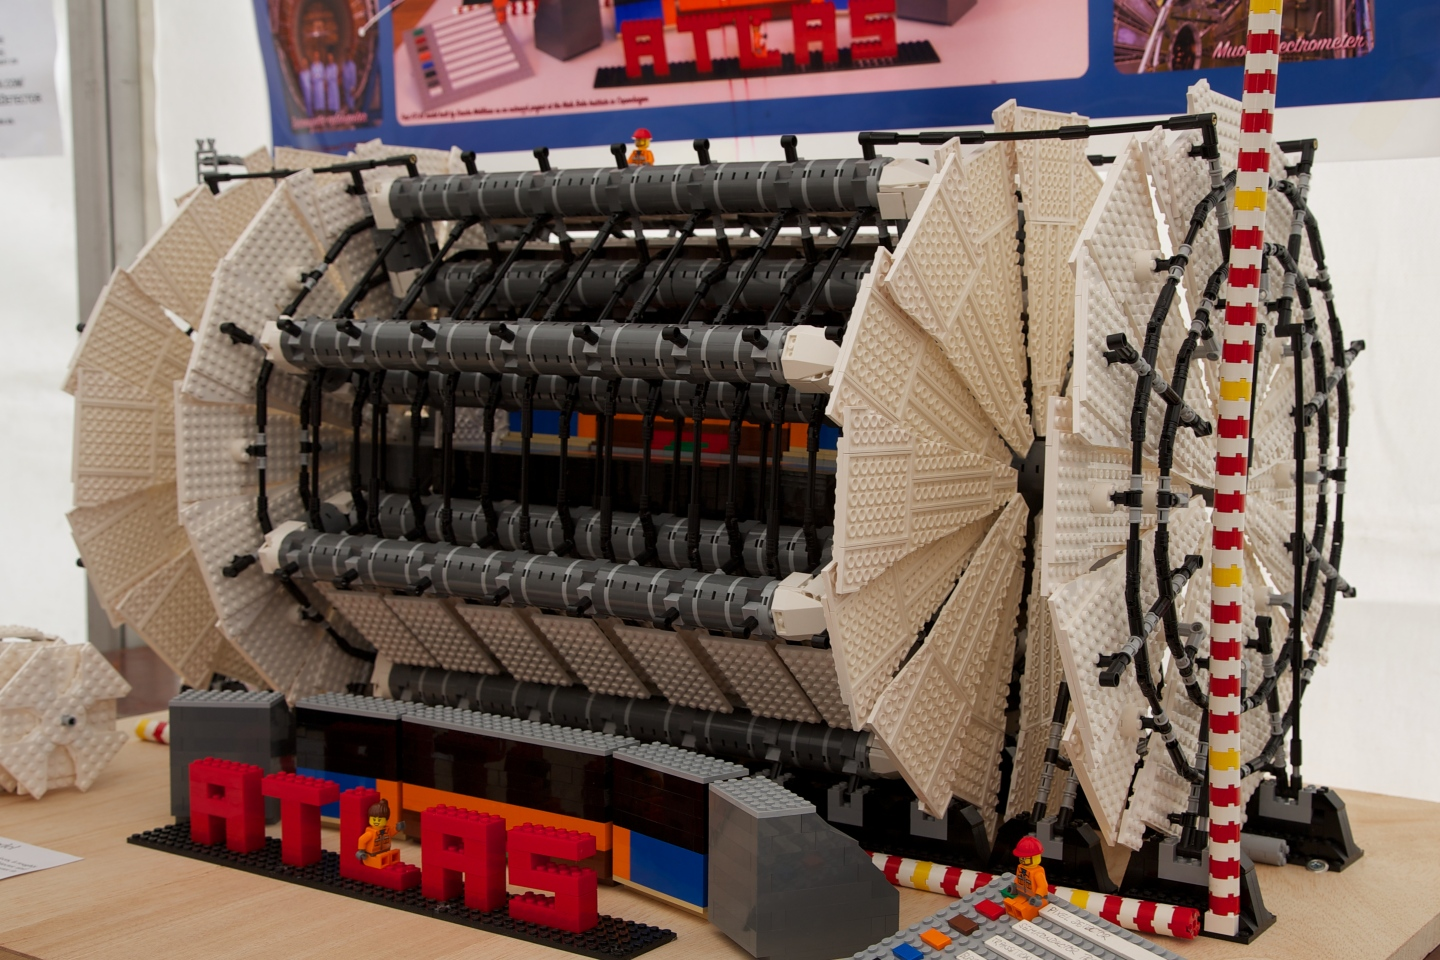
\includegraphics[width=\linewidth]{morelanguage/AtlasLego}
  \end{block}
\end{frame}

\begin{frame}[fragile]
  \frametitlecpp[98]{Using the STL}
  \begin{alertblock}{Exercise Time}
    \begin{itemize}
    \item go to code/stl
    \item look at the non STL code in randomize.nostl.cpp
      \begin{itemize}
        \item it creates a vector of ints at regular intervals
        \item it randomizes them
        \item it computes differences between consecutive ints
        \item and the mean and variance of it
      \end{itemize}
    \item open randomize.cpp and complete the ``translation'' to STL
    \item see how easy it is to reuse the code with complex numbers
    \end{itemize}
  \end{alertblock}
\end{frame}

\begin{frame}[fragile]
  \frametitlecpp[98]{Using the STL}
  \begin{alertblock}{Some last warning}
    You may find the STL quite difficult to use.
    \begin{itemize}
    \item template syntax is really tough
    \item it is hard to debug (compilers spit out long error novels)
    \end{itemize}
    However, this has improved a lot with \cpp11 \\
    And may again in \cpp20 with concepts
  \end{alertblock}
\end{frame}

\begin{frame}[fragile]
  \frametitlecpp[11]{Loops and auto keyword with the STL}
  \begin{block}{Old way}
    \begin{cppcode*}{}
      std::vector<int> v = ...;
      int sum = 0;
      for (std::vector<int>::iterator it = v.begin();
           it != v.end(); it++) {
        sum += *it;
      }
    \end{cppcode*}
  \end{block}
  \pause
  \begin{block}{New way}
    \begin{cppcode*}{firstnumber=7}
      std::vector<int> v = ...;
      int sum = 0;
      for (auto a : v) { sum += a; }
    \end{cppcode*}
  \end{block}
  \pause
  \begin{exampleblock}{STL way (\cpp17)}
    \begin{cppcode*}{firstnumber=10}
      std::vector<int> v = ...;
      int sum = std::reduce(v.begin(), v.end(), 0);
    \end{cppcode*}
  \end{exampleblock}
\end{frame}
